
\subsection{MULTI-SCALE MATCH CRITERION}
In the presented algorithm, the match criterion to track the target is based on the $PIV$ technique, 
where from two images a ROI and a Window Of Search ($WOS$) are defined. A target (object) is identified 
from the highest value of correlation ($PCC$) between a selected $ROI$ and a $WOS$, which determines an object's location.

Fig. \ref{fig:multires}(a) shows an application in two dimensions, where
the regions are compared with a ROI using the same scale.

The Fig. \ref{fig:multires}(b) reveals how the dimension of depth was included and
the search is made in different scales (layers). Similarly to the two dimension case, 
in three dimensions the target is also found through the highest $PCC$, but the object found may be 
bigger or smaller than the last target found.

\begin{figure}[H]
\centering
  \subfloat[]{\label{subfig:(a)} 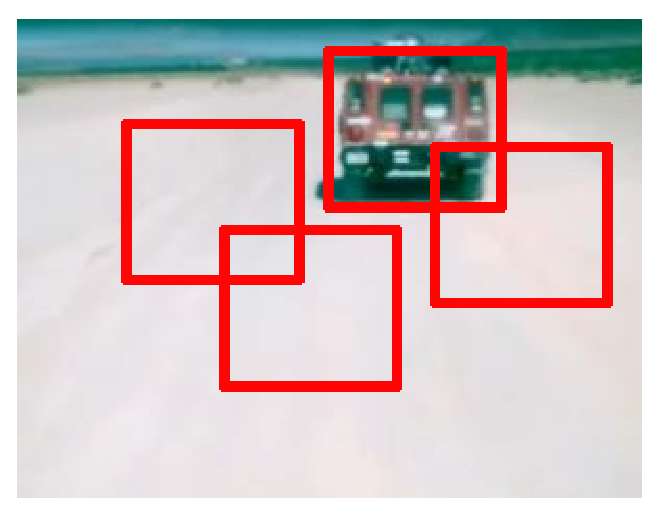
\includegraphics[width=.5\columnwidth]{images/figure2a.eps}}
  \subfloat[]{\label{subfig:(b)} 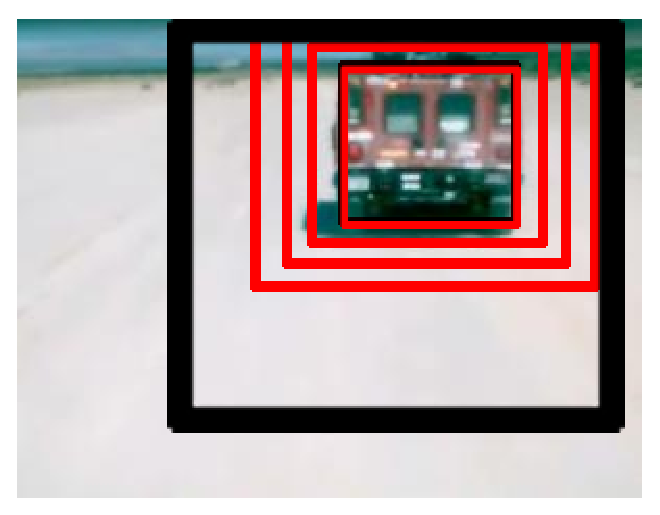
\includegraphics[width=.5\columnwidth]{images/figure2b.eps}}
  \caption{The red boxes show the analyzed regions and the black boxes represent the $WOS$. 
  (a) The regions are compared with a $ROI$ using the same scale. 
  (b) The regions are compared with a $ROI$ using different scales.}
  \label{fig:multires}
\end{figure}




%onde estava, onde esta agora
%que tamanho tinha que tamanho tem.